\documentclass[final]{article}

\usepackage{APS360}
\usepackage[utf8]{inputenc}
\usepackage[T1]{fontenc}
\usepackage{hyperref}
\usepackage{url}
\usepackage{booktabs}
\usepackage{amsfonts}
\usepackage{nicefrac}
\usepackage{microtype}
\usepackage{xcolor}
\usepackage{graphicx}
\usepackage{amsmath}
\usepackage{tikz}
\usetikzlibrary{arrows.meta, positioning}

\title{APS360 Final Report:\\Chunking Hit-Object Sequences in \texttt{.osu} Files Using Sequence Models}

\author{%
  Ben Lian \\
  1010943525, ben.lian@mail.utoronto.ca\\
  \url{https://github.com/dongdongben/Pattern-recognition-of-hit-objects-in-.osu-files}
}

\begin{document}

\maketitle

\vspace{-0.5in}

\section*{Introduction}
This project studies \emph{chunking} in the rhythm game \textit{osu!}. During play, notes are usually not read one at a time. Instead, players group nearby hit objects into short local reading units such as ``1-2-3'' or ``1-2-3-4.'' The goal of the project is to predict that structure directly from beatmap data. In the final version of the project, the model predicts whether each hit object starts a new chunk. Once chunk starts are predicted, within-chunk positions can be reconstructed by resetting to 1 at each predicted start and incrementing afterward.

This problem is interesting because it is both a game AI task and a perception task. Chunking depends on geometry, timing, and local sequence context rather than any one note in isolation. These relationships are difficult to describe with fixed rules, but they are well suited to learned sequence models. In addition, \textit{osu!} beatmaps are stored in a structured text format, so the data can be parsed reproducibly and converted into a supervised learning dataset.

\section*{Illustration}
\begin{figure}[!h]
\centering
\small
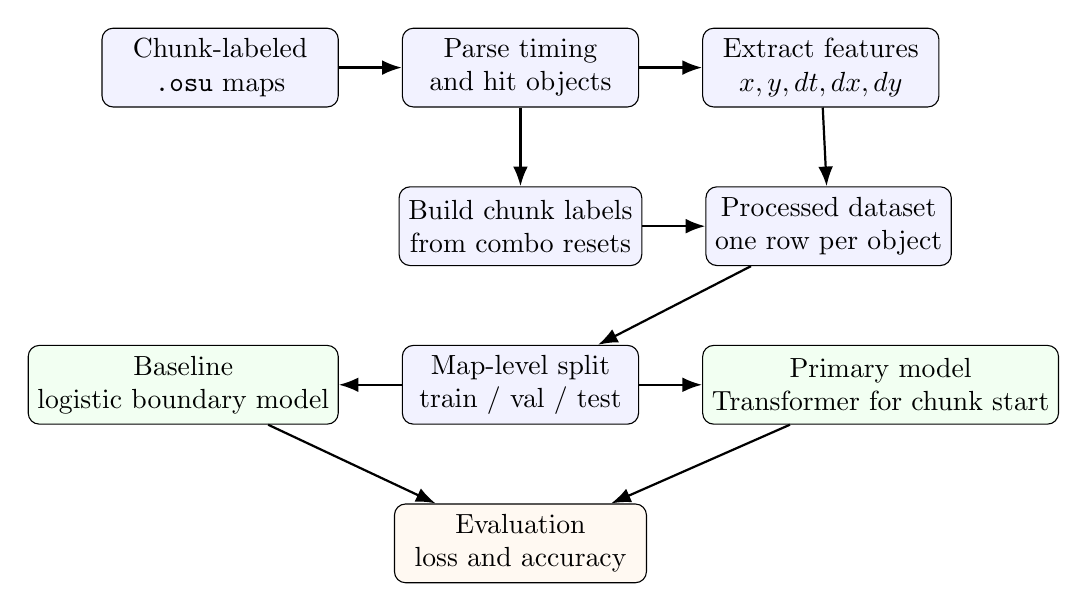
\begin{tikzpicture}[
    node distance=1.0cm and 0.8cm,
    box/.style={
        draw,
        rounded corners,
        minimum width=3.0cm,
        minimum height=1.0cm,
        align=center,
        fill=blue!5
    },
    modelbox/.style={
        draw,
        rounded corners,
        minimum width=3.2cm,
        minimum height=1.0cm,
        align=center,
        fill=green!5
    },
    evalbox/.style={
        draw,
        rounded corners,
        minimum width=3.2cm,
        minimum height=1.0cm,
        align=center,
        fill=orange!5
    },
    arrow/.style={-{Latex[length=2.5mm]}, thick}
]

\node[box] (raw) {Chunk-labeled\\\texttt{.osu} maps};
\node[box, right=of raw] (parser) {Parse timing\\and hit objects};
\node[box, right=of parser] (features) {Extract features\\$x,y,dt,dx,dy$};

\node[box, below=of parser] (labels) {Build chunk labels\\from combo resets};
\node[box, right=of labels] (dataset) {Processed dataset\\one row per object};

\node[box, below=of labels] (split) {Map-level split\\train / val / test};
\node[modelbox, left=of split] (baseline) {Baseline\\logistic boundary model};
\node[modelbox, right=of split] (transformer) {Primary model\\Transformer for chunk start};
\node[evalbox, below=of split] (eval) {Evaluation\\loss and accuracy};

\draw[arrow] (raw) -- (parser);
\draw[arrow] (parser) -- (features);
\draw[arrow] (parser) -- (labels);
\draw[arrow] (features) -- (dataset);
\draw[arrow] (labels) -- (dataset);
\draw[arrow] (dataset) -- (split);
\draw[arrow] (split) -- (baseline);
\draw[arrow] (split) -- (transformer);
\draw[arrow] (baseline) -- (eval);
\draw[arrow] (transformer) -- (eval);
\end{tikzpicture}
\caption{Overall system pipeline. Chunk-labeled beatmaps are parsed into hit-object sequences, converted into per-object geometric and temporal features, split at the map level, and used to train both a logistic baseline and a Transformer model for chunk-start prediction.}
\label{fig:system}
\end{figure}

\section*{Background \& Related Work}
Several prior works motivate this project. \textbf{TaikoNation} studies pattern-aware generation for rhythm games and shows that chart structure can be learned rather than hand-coded. \textbf{Mania Archetype} similarly focuses on rhythm-game chart organization and supports the idea that player-facing chart patterns can be represented statistically. \textbf{Osu2MIR} demonstrates that \textit{osu!}-derived data can be repurposed as a machine learning dataset rather than only a game artifact. Outside rhythm games specifically, survey work on \textbf{deep learning for procedural content generation} places chart understanding in a broader family of learned game-content tasks. Finally, \textbf{Attention Is All You Need} is directly relevant because the Transformer architecture is designed to model relationships across multiple positions in a sequence, which matches the chunking problem well.

These works are related, but not identical to the present project. Most prior rhythm-game papers focus on chart generation, timing, or broad chart structure. My project instead focuses on a reading-oriented problem: how hit objects should be grouped into locally readable units.

\section*{Data Processing}
The data source is a collection of chunk-labeled \texttt{.osu} beatmaps stored in \texttt{data/raw}. In these files, combo resets were manually edited so that each chunk begins at a note whose combo number is 1. The preprocessing script parses the \texttt{[TimingPoints]} and \texttt{[HitObjects]} sections of each beatmap and converts them into one row per hit object in a CSV dataset.

For every note, I compute absolute position \((x,y)\), elapsed time in milliseconds and beats (\texttt{dt\_ms}, \texttt{dt\_beats}), displacement from the previous note (\texttt{dx}, \texttt{dy}), Euclidean distance, normalized distance, and binary indicators for sliders and spinners. The final processed dataset contains \textbf{15 beatmaps} and \textbf{17{,}527} hit-object rows. The current map-level split contains \textbf{12{,}388} training rows, \textbf{2{,}333} validation rows, and \textbf{2{,}806} test rows. Splitting is performed by map rather than by row so that evaluation is done on unseen beatmaps instead of unseen notes from the same map.

The final feature vector contains the following 10 values:
\[
[x, y, dt_{ms}, dt_{beats}, dx, dy, distance, norm\_distance, is\_slider, is\_spinner].
\]
The chunk labels \texttt{chunk\_id} and \texttt{chunk\_pos} are preserved in the processed CSV, but the final model is trained only on the derived binary label \texttt{chunk\_start}.

\section*{Architecture}
My final neural architecture is a Transformer encoder that predicts \texttt{chunk\_start} rather than directly predicting \texttt{chunk\_pos}. This change was important. Earlier experiments treated \texttt{chunk\_pos} as a direct multiclass classification problem, but that formulation allowed structurally invalid outputs and ignored the fact that chunk positions must increase until a reset. Predicting chunk starts first is much more faithful to the real structure of the labels.

Each note feature vector is projected through a linear layer into a hidden dimension of \textbf{128}. I then add sinusoidal positional encoding so the model can distinguish early and late notes within a sequence. The encoder contains \textbf{2 Transformer blocks}, each with \textbf{4 attention heads} and a feedforward width of \textbf{256}. I use sequence length \textbf{8}, batch size \textbf{5}, AdamW optimization with learning rate \textbf{$3\times10^{-4}$}, weight decay \textbf{$10^{-4}$}, and gradient clipping at \textbf{1.0}. The model outputs a binary prediction per note: 1 if the note starts a new chunk, and 0 otherwise.

\section*{Baseline Model}
The baseline is a logistic chunk-boundary classifier implemented as a single linear layer with sigmoid output, which is equivalent to logistic regression. It predicts whether each hit object begins a new chunk using local geometric and temporal features. After boundary prediction, chunk positions can be reconstructed by resetting to 1 whenever a start is predicted and incrementing between starts.

This is a useful baseline because it is simple, fast to train, and easy to interpret. If the Transformer cannot outperform it, then either the chosen features are already highly informative under a linear rule or the neural model still needs more data to use its sequential capacity effectively.

\section*{Quantitative Results}
Table \ref{tab:results} summarizes the final quantitative results. The baseline was evaluated on the held-out test split. The Transformer checkpoint was selected using validation loss, and the saved best checkpoint was then evaluated on the held-out test split.

\begin{table}[!h]
\centering
\small
\begin{tabular}{lccc}
\toprule
Model & Split & Loss & Accuracy \\
\midrule
Logistic baseline & Test & -- & 85.00\% \\
Transformer & Validation (best) & 0.5195 & 73.38\% \\
Transformer & Test & 0.5768 & 70.06\% \\
\bottomrule
\end{tabular}
\caption{Final results reported using loss and accuracy only.}
\label{tab:results}
\end{table}

The baseline remained very competitive and achieved \textbf{85.00\%} test accuracy on chunk-start detection. The Transformer improved substantially after reformulating the target from \texttt{chunk\_pos} to \texttt{chunk\_start}, but its final held-out performance was lower than the baseline. The best validation checkpoint reached \textbf{73.38\%} validation accuracy with validation loss \textbf{0.5195}, and that checkpoint achieved \textbf{70.06\%} test accuracy with test loss \textbf{0.5768}.

\section*{Qualitative Results}
Qualitatively, both models identify chunk starts well when there is a strong local cue such as a large jump, a spacing reset, or a clear visual transition into a new pattern. The Transformer also handles some multi-note situations more naturally because it can attend across a short local sequence instead of relying only on the current note pair.

The most common failure cases occur in dense passages where chunking depends on subtle shape structure rather than an obvious local spacing change. In these cases, the model either inserts a boundary too early or misses one altogether. These failure modes are consistent with the current quantitative results: the final Transformer is learning a meaningful chunk-start signal, but its representation is still limited by the size and diversity of the dataset.

\section*{Evaluate Model on New Data}
To evaluate generalization on new data, all splits were performed at the \emph{map level}. This is critical for the project, since notes within the same map are highly correlated and a random row-level split would overestimate performance. In the current processed dataset, the final split contains 10 training maps, 2 validation maps, and 3 test maps.

The final Transformer result therefore reflects performance on beatmaps that were not seen during training. Although the test accuracy is lower than the baseline, the model still generalizes above chance and produces stable loss and accuracy on unseen maps. This makes the result meaningful as an evaluation of chunk-start prediction rather than memorization.

\section*{Discussion}
The most important lesson from this project is that the formulation of the target matters as much as the choice of model. Directly predicting \texttt{chunk\_pos} seemed natural at first, but it ignored the monotonic structure of chunk positions. Since chunk positions should increase until a reset, treating them as unconstrained classes made the learning problem unnecessarily hard and led to weaker results. Switching to \texttt{chunk\_start} made the task much more stable and interpretable.

At the same time, the final results show that model complexity alone is not enough. The logistic baseline outperformed the Transformer on the held-out test split. I do not view this as a failure; instead, it is an informative result. It suggests that with the current dataset and feature set, most of the learnable chunk-start signal is still strongly local. The Transformer likely needs either more maps, more diverse mapper styles, or stronger shape-aware features in order to make better use of its sequential capacity.

\section*{Project Difficulty / Quality}
I believe this project is reasonably challenging for the course scope. The task is not a standard image classifier or a simple sequence prediction problem. First, the target itself is somewhat subjective: chunking is intended to reflect reading behavior, not only a mechanical property of the chart. Second, the supervision is weak, since the labels are derived from edited combo structure rather than from a large set of independent expert annotations. Third, the output has real structure: chunk positions should increase monotonically and reset at the correct moments. Finally, the dataset is small compared with many deep learning projects, which makes cross-map generalization difficult.

Given those challenges, the project still produced a full preprocessing pipeline, a reproducible dataset, a strong baseline, a Transformer model, and a clear final comparison. Even though the Transformer did not surpass the linear baseline, the project demonstrates a complete applied machine learning workflow and surfaces a genuine insight: for this problem and dataset, target design and data representation matter more than simply increasing model complexity.

\section*{Ethical Considerations}
There are two main ethical considerations in this project. The first is data usage. \textit{osu!} beatmaps may be associated with copyrighted music and visual assets, so the project uses only the text-based \texttt{.osu} files and derived numerical features, not the audio or image files themselves. The second is label subjectivity. The chunk labels in this project reflect one reading interpretation encoded through edited combo structure, which means they may not match how all players would read the same map. The model should therefore be interpreted as an assistive or descriptive system, not as an authoritative definition of the one correct way to read a beatmap.

\newpage
\section*{References}
\begin{enumerate}
    \item Ash Vaswani et al. ``Attention Is All You Need.'' \emph{Advances in Neural Information Processing Systems}, 2017.
    \item Halina et al. ``TaikoNation: Patterning-Focused Chart Generation for Rhythm Games.'' 2021.
    \item Wang et al. ``Mania Archetype.'' 2024.
    \item Liu et al. ``Osu2MIR.'' 2025.
    \item Liu et al. ``Deep Learning for Procedural Content Generation.'' 2021.
    \item \textit{osu!} Wiki. ``File Format.'' \url{https://osu.ppy.sh/wiki/en/Client/File_formats/osu_(file_format)}.
    \item \textit{osu!} Wiki. \url{https://osu.ppy.sh/wiki}.
\end{enumerate}

\end{document}
